\documentclass{mimosis}

\usepackage{metalogo}
\setlength{\parindent}{0pt}

%%%%%%%%%%%%%%%%%%%%%%%%%%%%%%%%%%%%%%%%%%%%%%%%%%%%%%%%%%%%%%%%%%%%%%%%
% Some of my favourite personal adjustments
%%%%%%%%%%%%%%%%%%%%%%%%%%%%%%%%%%%%%%%%%%%%%%%%%%%%%%%%%%%%%%%%%%%%%%%%
%
% These are the adjustments that I consider necessary for typesetting
% a nice thesis. However, they are *not* included in the template, as
% I do not want to force you to use them.

% This ensures that I am able to typeset bold font in table while still aligning the numbers
% correctly.
\usepackage{etoolbox}

\usepackage[binary-units=true]{siunitx}
\DeclareSIUnit\px{px}

\sisetup{%
  detect-all           = true,
  detect-family        = true,
  detect-mode          = true,
  detect-shape         = true,
  detect-weight        = true,
  detect-inline-weight = math,
}

%%%%%%%%%%%%%%%%%%%%%%%%%%%%%%%%%%%%%%%%%%%%%%%%%%%%%%%%%%%%%%%%%%%%%%%%
% Hyperlinks & bookmarks
%%%%%%%%%%%%%%%%%%%%%%%%%%%%%%%%%%%%%%%%%%%%%%%%%%%%%%%%%%%%%%%%%%%%%%%%

\usepackage[%
  colorlinks = true,
  citecolor  = RoyalBlue,
  linkcolor  = RoyalBlue,
  urlcolor   = RoyalBlue,
  ]{hyperref}

\usepackage{bookmark}

%%%%%%%%%%%%%%%%%%%%%%%%%%%%%%%%%%%%%%%%%%%%%%%%%%%%%%%%%%%%%%%%%%%%%%%%
% Bibliography
%%%%%%%%%%%%%%%%%%%%%%%%%%%%%%%%%%%%%%%%%%%%%%%%%%%%%%%%%%%%%%%%%%%%%%%%
%
% I like the bibliography to be extremely plain, showing only a numeric
% identifier and citing everything in simple brackets. The first names,
% if present, will be initialized. DOIs and URLs will be preserved.

\usepackage[%
  autocite     = plain,
  backend      = bibtex,
  doi          = true,
  url          = true,
  giveninits   = true,
  hyperref     = true,
  maxbibnames  = 99,
  maxcitenames = 99,
  sortcites    = true,
  style        = numeric,
  ]{biblatex}

\input{bibliography-mimosis}
\bibliography{Thesis}

%%%%%%%%%%%%%%%%%%%%%%%%%%%%%%%%%%%%%%%%%%%%%%%%%%%%%%%%%%%%%%%%%%%%%%%%
% Fonts
%%%%%%%%%%%%%%%%%%%%%%%%%%%%%%%%%%%%%%%%%%%%%%%%%%%%%%%%%%%%%%%%%%%%%%%%

\ifxetexorluatex
  \setmainfont{Minion Pro}
\else
  \usepackage[lf]{ebgaramond}
  \usepackage[oldstyle,scale=0.7]{sourcecodepro}
  \singlespacing
\fi

\renewcommand{\th}{\textsuperscript{\textup{th}}\xspace}

\newacronym[description={Principal component analysis}]{PCA}{PCA}{principal component analysis}
\newacronym                                            {SNF}{SNF}{Smith normal form}
\newacronym[description={Topological data analysis}]   {TDA}{TDA}{topological data analysis}

\newglossaryentry{LaTeX}{%
  name        = {\LaTeX},
  description = {A document preparation system},
  sort        = {LaTeX},
}

\newglossaryentry{Real numbers}{%
  name        = {$\real$},
  description = {The set of real numbers},
  sort        = {Real numbers},
}

\makeindex
\makeglossaries

\usepackage{minted}
\usepackage{tikz}
\usetikzlibrary{snakes,arrows,shapes}
\usepackage[pdf]{graphviz}
\usepackage{amsfonts}

%%%%%%%%%%%%%%%%%%%%%%%%%%%%%%%%%%%%%%%%%%%%%%%%%%%%%%%%%%%%%%%%%%%%%%%%
% Incipit
%%%%%%%%%%%%%%%%%%%%%%%%%%%%%%%%%%%%%%%%%%%%%%%%%%%%%%%%%%%%%%%%%%%%%%%%

\title{\texttt{latex-mimosis}}
\subtitle{A minimal, modern \LaTeX{} package for typesetting your thesis}
\author{Bastian Rieck}

\begin{document}

\frontmatter
  \begin{titlepage}
  \vspace*{5cm}
  \makeatletter
  \begin{center}
    \begin{Huge}
      \@title
    \end{Huge}\\[0.1cm]
    %
    \emph{by}\\
    \@author
    %
    \vfill
    Advisor: Malchiodi Dario \\
    Co-advisor: Cesa-bianchi Nicolo' \\
    Fall 2018
  \end{center}
  \makeatother
\end{titlepage}

\newpage
\null
\thispagestyle{empty}
\newpage

  \include{Sources/Abstract}

  \tableofcontents

\mainmatter

  %%%%%%%%%%%%%%%%%%%%%%%%%%%%%%%%%%%%%%%%%%%%%%%%%%%%%%%%%%%%%%%%%%%%%%%%
\chapter{Technology}
%%%%%%%%%%%%%%%%%%%%%%%%%%%%%%%%%%%%%%%%%%%%%%%%%%%%%%%%%%%%%%%%%%%%%%%%

In this chapter I'm describing the technology that I used to implement
the set of utilities and experiments described in section ??? This
chapter is organized as follows. In \ref{sec:tensorflow} I'm describing
what is TensorFlow and how its computational graphs work. In
\ref{sec:keras} I'm describing Keras, an high-level API for building
Machine Learning models without working with a low-level library like
TensorFlow. In \ref{sec:cleverhans} I'm describing CleverHans, a
library to generate adversarial examples against a given model. In
\ref{sec:sklearn} I'm describing scikit-learn, a library for building
and training Machine Learning models.

\section{TensorFlow}
\label{sec:tensorflow}

TensorFlow is a C++ framework for Machine Learning released by Google.
It uses a programming model called Data Flow that aims to allow
distributed and parallel computations. While this \emph{paradigm} makes
TensorFlow suitable even for research and production environments, it
can be quite daunting to use when tinkering. In fact, computational
graphs are built and only later executed. This is counter-intuitive at
first. In the following example,

\begin{minted}{python}
  >>> import tensorflow as tf
  >>> symbol = tf.constant(42)
  >>> symbol 
  <tf.Tensor 'Const:0' shape=() dtype=int32>
\end{minted}

\texttt{symbol} doesn't contain a reference to the integer 42. Instead
it contains a reference to a node of the computational graph (which
will always output 42). In general until you don't run the
computational graph it's hard to determine what's going to be the value
of a tensor. This is slowing down exploratory analysis.

\subsection{About computational graphs}
\label{subsec:computational-graph}

TensorFlow computational graphs are an important part of the framework.
A computational graph is a directed graph representing a computation
involving tensors. A tensor in TensorFlow is a multi-dimensional array:
it can be a scalar, a matrix, a batch of RGB images (a 4D vector), ...
Each node represents an operation on tensors while edges represent
tensors.

Figure \ref{fig:easygraph} shows the graph associated to an addition of
two \texttt{tf.float32}'s (i.e. two tensors made of 32-bit float
numbers). The first two nodes \texttt{a} and \texttt{b} outputs a
tensor each. Those are used to feed the \texttt{add} node that will
output the tensor resulting from the sum of \texttt{a} and \texttt{b}.
Note that tensors are associated with edges only. Yet, a node can
perform the operation of just \emph{returning} a tensor.

\begin{figure}[H]
  \centering
  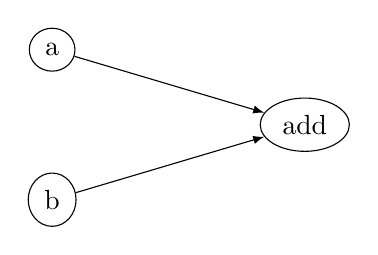
\begin{tikzpicture}[>=latex,line join=bevel,]
  \node (a) at (27.0bp,72.0bp) [draw,ellipse] {a};
    \node (add) at (117.95bp,45.0bp) [draw,ellipse] {add};
    \node (b) at (27.0bp,18.0bp) [draw,ellipse] {b};
    \draw [->] (b) ..controls (61.417bp,28.218bp) and (72.527bp,31.516bp)  .. (add);
    \draw [->] (a) ..controls (61.417bp,61.782bp) and (72.527bp,58.484bp)  .. (add);
  \end{tikzpicture}
  \caption[easygraph]{An easy computational graph}
  \label{fig:easygraph}
\end{figure}

The code to build the graph of Figure \ref{fig:easygraph} using the
TensorFlow Python API is

\begin{minted}{python}
  >>> import tensorflow as tf
  >>> a = tf.placeholder(tf.float32)
  >>> b = tf.placeholder(tf.float32)
  >>> add = tf.add(a, b)
  >>> add
  <tf.Tensor 'add:0' shape=<unknown> dtype=float32>
\end{minted}

\section{Keras}
\label{sec:keras}

Keras is a high level library for building Machine Learning models. It consists
of a simple API and bindings for a backend of choice, most notably TensorFlow.
When you use the library, you're encouraged to use \emph{layers} instead of
plain tensors. In fact the whole concept of TensorFlow tensors is hidden away by
the library abstractions. To implement your model you stack layers. For example,
you would stack a \texttt{Dense} layer and an \texttt{Activation} one to
implement a simple neural network.

\begin{minted}{python}
  from keras.models import Sequential

  model = Sequential([
    Dense(batch_input_shape=(None, 784), 10),
    Activation('softmax')
  ])
\end{minted}

Under the hood, a \texttt{Layer} is simply a callable object whose
\texttt{\_\_call()\_\_} method takes a TensorFlow tensor \texttt{X} and
manipulates it. For example a simple custom one would be
\begin{minted}{python}
  from keras.engine.base_layer import Layer
  import tensorflow as tf

  class Add42(Layer):
      def __init__(self):
          self.fortytwo = tf.constant(42)

      def __call__(self, X):
          return tf.add(X, self.fortytwo)
\end{minted}

While the idea is clean and beginner friendly, at the time of this writing the
abstraction can become leaky when things goes wrong, needing the programmer to know
about TensorFlow computational graphs to debug her program successfully.

\section{CleverHans}
\label{sec:cleverhans}

CleverHans is a library written by Google for building adversarial examples. It
implements a variety of attacks against neural networks (FGS, T-FGS, Carlini and
Wagner, ...) and it's compatible with models built with Keras. It uses the same
computational graphs of TensorFlow to generate adversarial examples; again, as
you use the library more and more understanding computational graphs becomes a
necessity.

\section{Scikit-learn}
\label{sec:sklearn}

Scikit-learn is a Python library written by Google providing a number of models,
learning algorithms and other utilities for Machine Learning. It's perfect for
fast prototyping as it uses a simple and consistent API and handles numpy arrays
or even Python lists.

I've used scikit-learn to borror a couple of decomposition algorithms (PCA, FastICA, ...)
without having to implement them. This required a bit of reasoning as reusing scikit-learn algorithms on
TensorFlow graphs was not straightforward.


% This ensures that the subsequent sections are being included as root
% items in the bookmark structure of your PDF reader.
\bookmarksetup{startatroot}
\backmatter

  \begingroup
    \let\clearpage\relax
    \glsaddall
    \printglossary[type=\acronymtype]
    \newpage
    \printglossary
  \endgroup

  \printindex
  \printbibliography

\end{document}
